\documentclass[oneside]{memoir}
\usepackage[utf8]{inputenc}
\usepackage[ngerman]{babel}
\usepackage[T1]{fontenc}
\usepackage{lettrine}
\usepackage{hyperref}
\usepackage{graphicx}
\DisemulatePackage{setspace}
\usepackage{setspace}
\onehalfspacing

\newcommand{\parasep}{
\bigskip
\bigskip
\begin{center} 
   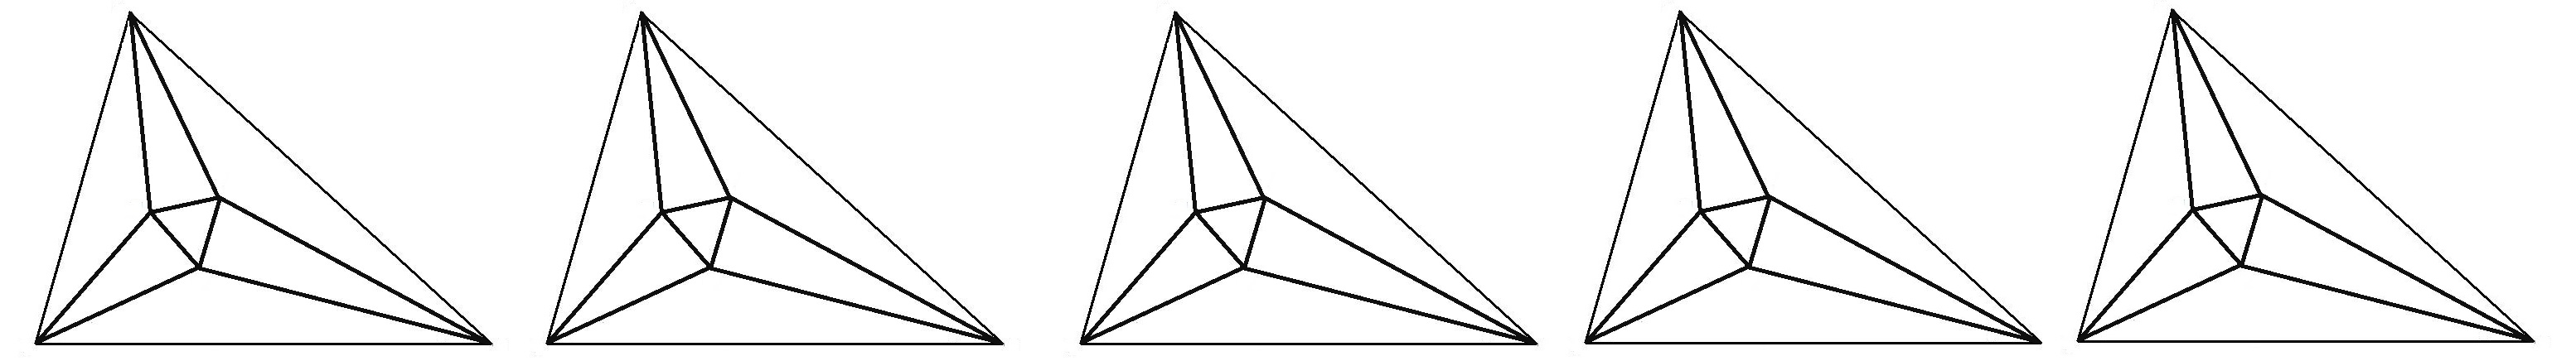
\includegraphics[scale=.08]{parasep5.jpg} 
\end{center}
\bigskip
\bigskip
}

\makeatletter
\newenvironment{chapquote}[2][2em]
  {\setlength{\@tempdima}{#1}%
   \def\chapquote@author{#2}%
   \parshape 1 \@tempdima \dimexpr\textwidth-2\@tempdima\relax%
   \itshape}
  {\par\normalfont\hfill--\ \chapquote@author\hspace*{\@tempdima}\par\bigskip}
\makeatother
\pretitle{\begin{center}\Huge\bfseries}
\title{Lockdown}
\posttitle{\par\vskip1em{\normalfont\normalsize\scshape Eine AIMO-Geschichte\par\vfill}\end{center}}
\author{Herausgegeben von einer nichtleeren Teilmenge der AIMO-Teilnehmer 2020}
\predate{\vfill\begin{center}\large}
\begin{document}
\begin{titlingpage}
\maketitle
\end{titlingpage}
\newpage
\thispagestyle{empty}
\begin{center}
\fbox{\parbox{0.8\textwidth}{\textbf{Disclaimer.} \hspace{0.2cm} Dies ist eine Fanfiction, das heißt, eine erfundene Geschichte, die in Anlehnung an die Geschehnisse der AIMO 2020 geschrieben wurde. Alle vorkommenden Handlungen sind rein fiktiv, insbesondere besteht kein Zusammenhang zwischen den realen und erfundenen Handlungen bestimmter Charaktere.}}
\end{center}
\setcounter{page}{2}
\chapter{Prolog in der Hölle}

\begin{chapquote}{Fyodor Dostoevsky}
\glqq Aus hundert Kaninchen wird niemals ein Pferd und aus hundert Verdachtsgründen niemals ein Beweis.\grqq
\end{chapquote}

\lettrine{M}{arc Hieke} schaute müde von den zahlreichen Mathematikaufgaben vor sich wieder auf. Links und rechts in seinem Blickfeld stapelten sich Blätter, und er seufzte. Das spärliche, flackernde Licht einer Glühbirne erleuchtete matt das Zimmer, in dem außer dem Tisch keine Möbel standen. Genauso wenig gab es Fenster -- Marc vermisste das Sonnenlicht schon seit Längerem. Seit Stunden versuchte er sich an einer Zahlentheorieaufgabe und kam nicht voran. Sein Kopf schmerzte. Als er Schritte vor seiner vergitterten Tür hörte, begann sein Puls zu rasen. Die Tür schwang auf und eine in einem dunklen Umhang verhüllte Figur erschien. Sie holte aus ihrem Umhang einen weiteren Stapel hervor und knallte ihn vor Marc. \\
„Die sind bis morgen erledigt, sonst gibt's kein Essen.“ \\
Marc schluckte. Die Figur ging wieder in Richtung Tür. Der Umhang flatterte, und darauf prangte ein aufgesticktes Symbol. Die Winkeldreiteilenden eines Dreiecks, die ein weiteres, gleichseitiges Dreieck bildeten. Das Morley-Dreieck.
\begin{figure}[htbp] 
  \centering
     \includegraphics[scale=0.6]{Bilder/morleycrop.png}
  \caption{Die geheimnisvolle Figur}
\end{figure}

\chapter{Definitionen und Grundbegriffe} %bis 1.5
\begin{chapquote}{Patrick Nasri-Roudsari}
\glqq Mal sehen schreib‘` ich die Fanfiction mit: Hat Jesus die Bibel geschrieben?\grqq
\end{chapquote}

\textit{Der 20. April 2020} \\ 
\lettrine{D}{ie Teilnehmerliste} auf der rechten Seite von Georgis Bildschirm füllte sich langsam, als Jürgen Prestin einen AIMO-Teilnehmer nach dem anderen in die Zoomsitzung ließ. Er gedachte, während dieser die am Abend davor abgeschickten Aufgaben zu besprechen. Die ihm inzwischen vertrauten Namen purzelten geradezu in die Sitzung, schon drei Minuten nach 16 Uhr waren so gut wie alle anwesend. Georgi nahm einen Schluck von der Tüte Orangensaft neben seinem Laptop und setzte seine Kopfhörer auf. Veran, Christian und Patrick waren bereits auf einem separaten Discordserver, in dem sie für gewöhnlich während den Seminaren ratschten – er beeilte sich und trat diesem bei. \\
„Und nach dem Eisensteinkriterium ist $P$ irreduzibel, glaube ich“, beendete Christian seinen Gedanken, woraufhin Veran zögernd sein Einverständnis gab. \\
„Hi“, sagte Georgi und erhielt einen Gruß von den beiden anderen. „Wo ist Patrick?“ \\
„Unklar“, antwortete Veran schroff. „Wahrscheinlich spielt er gerade GTA oder so.“
Ein Rauschen war von Patricks Mikrofon zu hören. Vermutlich hatte er sich gerade hingesetzt. \\ 
„Jungs, ich hab‘ mir grad so dick n Salat geholt“, gluckste Patrick vergnügt. „Meine Mutter hat wieder welche gekauft.“
Georgi wollte etwas dazu sagen, als sich Jürgen Prestin meldete. Er werde nun anfangen, ohne auf die Nachzügler zu warten. Es fehlte nur noch Marc, der schon die letzten paar Seminare hatte sausen lassen. Keiner der vieren wusste, ob er sich entschuldigt hatte oder warum genau er nicht erschien. Der Dozent fragte, wer denn zuerst eine Aufgabe vorstellen möchte, und während Georgi gerade darüber nachdachte, ob er die zwei Aufgaben, die er vorbereitet hatte, jetzt oder später vorstellen wollte, klinkte sich Christian aus dem Discord aus, hob auf Zoom seine Stummschaltung auf und fing an, über die 5 zu referieren. 
Nachdem er fertig war, trat er dem Channel mit den anderen wieder bei.  \\
„Voll kreativ“, lobte ihn Veran, worauf Christian sich bedankte. Er fragte daraufhin die anderen beiden im Call, ob sie die Aufgabe ähnlich gelöst hatten. \\
„Bruder, ich hab‘ grad gar nicht aufgepasst“, erwiderte Patrick leicht aufgebracht. „Es hat mich wieder dieser komische Typ angerufen.“ \\
„Der Nummernachbar?“, fragte Georgi. Der Unbekannte mit derselben Nummer wie Patrick bis auf die letzte Ziffer hatte ihn bereits vor dem ersten Bad Homburg-Seminar kontaktiert und hatte nur wirres Zeug von sich gegeben. Obwohl Sofia und die anderen sich über Michael, so hatte er sich genannt, lustig machten, war er Patrick ganz und gar nicht geheuer. \\
„Ja“, antwortete Patrick. „Er war aufgeregt und hat irgendwas davon geredet, dass ich vorsichtig sein sollte. Ich hab‘ einfach aufgelegt, ich fand das zu seltsam.“ \\
„Fishy“, sagte Christian. „Ich glaube, du brauchst das nicht allzu ernst nehmen.“ \\
„Ja, glaub‘ ich auch nicht“, meinte Patrick und richtete seine Aufmerksamkeit auf seinen Salat. „Der Typ ist sowieso nicht ganz klar im Kopf.“

%1.2.
\parasep

Veran stöpselte sich die Kopfhörer aus den Ohren. „Crko dabogda\footnote{möge ich nur sterben}, was für ein langweiliges Seminar“, dachte er sich -- tatsächlich hätte man die letzte Geo mithilfe von Inversion am Kreis kinderleicht i.t.s.-n können, anstatt sich stundenlang anhören zu müssen, wie Lennart Grabbel sie durchmüllert oder durcherict, je nachdem wie man es bezeichnet. Aus dem Nebenzimmer war schon das alltägliche Gestreite zwischen Verans Mutter, Verans Vater und Verans Bruder zu hören. \\
„Koji ćevapi, mrzim ćevape!\footnote{Was für Cevapcici, ich hasse Cevapcici!}“, schrie Verans Bruder. \\
„Juče si obavezno hteo da praviš sunce od tih ćevapa i čak si zvao sestru da je pitaš kako se pravi!\footnote{Gestern wolltest du da noch unbedingt eine Cevapcicisonne draus machen und hast dafür extra deine Cousine angerufen, damit sie dir sagt wie mans richtig macht!}“, schrie Verans Vater zurück. \\
„Mrzim vas sve!\footnote{Ich hasse euch alle!}“, schrie Verans Mutter und weinte. Veran hasste ebenso seine Familie, besonders wenn sie sich stundenlang streiten musste, deshalb entschied er sich raus an die frische Luft zu gehen um sich von dem serbischen Geschreie zu erholen. Er öffnete die Wohnungstür und blickte auf die tiefe, breite, sogar etwas furchterregende Treppe. Aber weit kam er nicht, denn seine Mutter hielt ihn auf. \\
„Gde ideš?\footnote{Wohin gehst du?}“, fragte sie skeptisch. \\
„Nigde\ldots\footnote{Nirgendwohin\ldots}“, murmelte Veran. Veran hatte keine Lust sich bei seiner Mutter zu rechtfertigen und beschloss sie lieber vom Thema abzulenken. „Ima seminar u Oberwolfachu za tri nedelje\footnote{In 3 Wochen ist Seminar in Oberwolfach.}“, sagte er. „Dabogda ti se visine u trouglu ne sekle u jednoj tački!\footnote{Mögen sich deine Höhen im Dreieck nicht in einem Punkt schneiden!}“, entsetzte sich Verans Mutter. Veran ignorierte sie und bahnte sich den Weg duchs Wohnzimmer zum Klavier um den Aufschwung zu spielen. Nur so konnte man nämlich die liebliche Stimme des serbischen Vizepräsidenten im Fernsehen, der Ausschau nach einer Karriere als Präsident hielt, übertönen. Sein sympathisches Gesicht bedeckte schon seid mehreren Tagen ununterbrochen das Fernsehapparat. Veran setzte sich ans Klavier und schwang auf. Wenn er spielte, vergaß er alles um sich herum: seine weinende Mutter, seinen meckernden Bruder, Vizepräsident Vučić, selbst seine Cousine, zu der man sogar sagen könnte, dass er eine besondere Beziehung hatte. Man könnte sagen, er reiste in eine andere Welt -- oder sogar in eine andere Zeit.

\parasep

\textit{Der 21. April 2020} \\ 
„Der Nummernnachbar von Patrick hat sich übrigens wieder gemeldet.“ Georgi telefonierte gerade mit seinem Freund Maximilian Keßler, welcher in den zwei Jahren zuvor an der AIMO teilgenommen und es 2019 auch zur IMO geschafft hatte, und berichtete ihm eifrig über die neuesten Geschehnisse. \\
 „Oh echt? Ich dachte der hätte längst aufgehört, Patrick zu schreiben?“, wunderte sich Max. \\
 „Ja, das letzte Mal haben wir in Bad Homburg von ihm gehört. Aber gestern während dem AIMO-Meeting hat er wieder bei Patrick angerufen\ldots“ Georgi erzählte ihm also alles über den mysteriösen Anruf. \\
 „Eure AIMO ist echt witzig, so etwas ist letztes und vorletztes Jahr nicht passiert!“, meinte Max Keßler daraufhin amüsiert. \\
 „Ja, das stimmt“, fand auch Georgi. „Aber dafür konntest du immerhin zu den Seminaren in Reallife fahren\ldots“ \\
  „Oh ja, vor allem die Woche in Oberwolfach hätte ich dir auch gegönnt!“ \\
   „Jaa, Corona ist echt so eine Bitch.“ \\
    „Ich sag‘ mal so, is nicht schön, aber wat willste machen?“, scherzte Max daraufhin und beide schmunzelten. Georgi erzählte weiter: \\
    „Aber mal im Ernst, die Zoom-Meetings sind einfach nicht das gleiche Erlebnis. Ich würde mich so langweilen, wenn ich nicht währenddessen mit den anderen über Discord reden würde. Marc zum Beispiel kommt seit einigen Tagen gar nicht mehr zu den Seminaren\ldots“ \\
    „Marc Hieke?“, fragte Max nach. \\
     „Ja“, bestätigte Georgi. \\
     „Fishy. Gerade der sollte sich doch mal bisschen mehr anstrengen. Seine Platzierung auf der Schätzliste sieht im Moment gar nicht gut aus“, bemerkte Max. Georgi stimmte ihm zu, und nach einigen weiteren Diskussionen über die Schätzliste und die Seminare klopfte es an Georgis Tür und man hörte seine Mutter rufen: „Essen ist fertig!“ \\
     „Ah, ich muss dann wohl gehen“, sagte Georgi zu Max. \\
     „Dann guten Appetit!“, antwortete Max und die beiden verabschiedeten sich.
     
\parasep

%1.5
\textit{Der 24. April 2020} \\ 
Unter dem blauroten Licht der großen Serbienfahne, die über dem Bett in Sofias Zimmer hing, hörte man ein lautes, verstörendes Lachen, das die im Nebenzimmer schlafende Mutter aufweckte. Sie dachte, ihre Tochter sei verrückt, allein wegen der Tatsache, dass ihr Zimmer von lauter „Serbien“ nicht atmen konnte. In Sofias Zimmer gab es nämlich, neben ihrem Lieblingskleid -- der serbischen Nationaltracht -- sowie der Flasche mit 89\%igem echten serbischen Pflaumenschnaps, tausende -- teilweise sehr nationalistische -- Bilder, die Symbole, Sprüche, Gegenstände aus und über Serbien beinhalteten und Sofia so sehr faszinierten. Ihr dortiger Aufenthalt im Jahr zuvor hat in ihr eine enorme Begeisterung für das Land ausgelöst -- sie werde eines Tages dort wohnen, sagte sie immer. \\
Auch in ihrem Telefonat mit Maria durften Serbienandeutungen nicht fehlen. Es war die Rede von einem „allgemeinen Beispiel“ sowie von einer ominösen „Person A“. Dabei wollte Maria nur wissen, welchen Zug Sofia für das Seminar in Oberwolfach nimmt\ldots \\ 
„Ich nehm‘ den um 08:49. Dann musst du aber sehr früh aufstehen\ldots“  \\ 
„Kein Problem“, antwortete Maria. „Ich wach‘ jeden Tag um Viertel vor sechs auf.“ \\  
„Du könntest aber auch die Nacht davor bei mir übernachten, meine Mutter hätte nichts dagegen“, schlug Sofia vor.  \\ 
„Hmm, ich bin mir nicht sicher\ldots“, sagte Maria. „Meine Mutter ist grad nicht da\ldots“  \\ 
„Du kannst doch deinen Vater fragen“, fiel Sofia ein. 
Doch Maria reagierte darauf sehr zögernd, und Sofia verstand sofort, dass es ein Fehler war, das gesagt zu haben. \\ 
„Ich habe keinen Vater“, erklärte Maria. „Ich hab ihn seit meiner Geburt nie kennengelernt\ldots{} und meine Mutter wollte nie darüber mit mir sprechen“. \\
„Fishy“, sagte Sofia darauf. 
Es folgten paar Sekunden Stille. 
 \\ 
„Ich bring‘ Marzipan zum Seminar mit“,  sagte Maria, um vom Thema abzulenken. \\
„Jaaa“, jubelte Sofia.  \\ 
„Wobei \ldots{} fuck! Jebote! Marzipan beginnt mit M!“  \\ 
„Und das heißt \ldots?“, reagierte Maria verwirrt.  \\ 
„Alle schlechten Dinge beginnen mit M!“, antwortete Sofia voller Euphorie. „Das ist Teil von meiner neuen Lebenseinstellung! Aber keine Sorge, du beginnst nicht mit M, weil Maria Matthis hat ja zwei M, und das hebt sich auf.“  \\ 
„Ah ja“, antwortete Maria und war noch einmal verstört von Sofias seltsamen Aussagen.  \\ 
„Ne Spaß, ich mag Marzipan“, beruhigte sie Sofia, nachdem sie gemerkt hatte, dass sie wieder einmal etwas übertrieben hat.
„Sorry, ich glaub‘ ich hab‘ wieder zu viel Tee gegessen.“ \\
Ab dem Moment wusste keine der beiden mehr, was sie sagen sollten.  \\ 
„Ich denke, ich muss jetzt schlafen gehen“, entschloss sich Maria. \\
„Ok\ldots“, sagte Sofia, „Gute Nacht.“ \\ 
„Gute Nacht“, sagte auch Maria und stürzte sich ins Bett. 
Es erwarteten sie wieder aufregende Träume.
     
     \parasep
     
%1.3
\textit{Der 25. April 2020} \\
Christian erwachte aus unruhigen Träumen. Wie immer ließ er sich davon aber nicht ablenken und als die ersten paar Strahlen der Münchner Sonne in sein Gesicht schienen, wurde ihm sofort klar: Es ist ein perfekter Tag zum Baden!
So verlor er keine einzige Sekunde und führte in größter Eile seine gewöhnliche Morgenroutine durch.
Nachdem er dann schnell, aber sorgfältig seine Zähne geputzt, geduscht, seine Badesachen angezogen, sich mit Sonnencreme eingeschmiert (obwohl es draußen nur 20 Grad heiß war), dann mit seiner Familie nach einem kurzen Gebet ein paar Semmeln und Brezn gefrühstückt und danach kurz den „QED-Chat“ gecheckt hatte, begab er sich auf eine wilde Fahrt zum Englischen Garten.
Er fuhr blitzschnell durch die Straßen von Schwabing, überquerte die Leopoldstraße und ließ sich dabei nicht von den Menschenmengen ablenken, die den schönen Tag in der Münchner Innenstadt verbringen wollten. Als er dann am großen Park ankam, wurde es schon etwas unangenehm, und das Fahrradfahren durch die mit Fußgängern gefüllten Wege war fast unmöglich. Obwohl dies für Christian eigentlich kein Problem darstellte, beschloss er diesmal, einen Umweg zu fahren -- bis zum Eisbach war es schließlich nicht mehr so weit.
Er fuhr dann Richtung Norden und entdeckte Teile des Parks, in denen er noch nie gewesen war. Die Bäume wurden immer dichter und der Himmel bewölkter. Christian bekam langsam Zweifel, ob der Weg, den er fuhr, sicher der Richtige sei, allerdings blieb er recht zuversichtlich -- den großen Eisbach könne er schließlich nicht verpassen.
Nach einigen Metern merkte er aber, dass mit seinem Fahrrad irgendwas nicht stimmte. Es machte seltsame Geräusche und fuhr nur noch sehr langsam. Er beschloss, es zu schieben, bis er eine größere Straße erreichen würde. Doch die Wege wurden immer enger und Christian verlor seine Orientierung. Von anderen Menschen war mittlerweile nichts mehr zu sehen. Die ersten Regentropfen fingen an zu fallen.
Christian hatte keine Kraft mehr. Als dann eine Herde von Enten die Straße überquerte, wurde ihm der Weg komplett versperrt.  \\
Christian blieb stehen.
Der Regen wurde immer stärker. \\
Und dann spürte er hinter seinem Rücken eine menschliche Gestalt, die ihm immer näher kam.
Er hörte eine bekannte Stimme. \\
„Guten Tag, Herr Noaghiu“, sagte sie.
Christian erstarrte.
 

\chapter{Einleitende Überlegungen} %bis 1.9
\begin{chapquote}{Sören Kierkegaard}
\glqq Wie ist doch die ganze Natur so ominös! Voll Vorbedeutung ist mir der Vögel Flug, ihr Schrei, der Fische ausgelaßnes Schlagen gegen die Oberfläche des Wassers, ihr Verschwinden in der Tiefe, fernes Hundegebell, eines Wagens fernes Gerassel, Schritte, die von fernher widerhallen. Nicht sehe ich Gespenster in dieser nächtlichen Stunde, nicht sehe ich, was war, sondern das, was kommen wird.\grqq
\end{chapquote}

%1.6
\textit{Der 26. April 2020} \\ 

     
\parasep
%1.7

\textit{Der 30. April 2020} \\
Es war Donnerstag, der 30. April 2020, der 42. Frühlingstag, und 12:36 am Nachmittag. Herr Prestin saß gedankenversunken an seinem Schreibtisch, seine Katze strich ihm um die Beine, und aus der Küche war leise das Radio zuhören, auf dem NDR Info gerade von dem neuen Antikörpertest berichtete, der eine Genauigkeit von über 99 Prozent haben solle. Doch das interessierte Herrn Prestin nicht, denn neben dem Vorbereitungsmaterial für die Erstsemester befanden sich auf seinem Schreibtisch einige sehr staubige Dokumente, die er soeben aus dem Keller geholt hatte. Sie waren noch aus seiner eigenen Studienzeit, unter anderem gab es dort ein Foto, welches in mit seinem Kommilitonen und guten Freund Michael kurz vor dem Abschluss zeigt. Die Erinnerung stimmte Herrn Prestin sentimental. Nichtsdestotrotz musste er es jetzt zusammen mit den Aufzeichnungen zum Morley-Dreieck (kurioserweise enthielten diese neben normalen geometrischen Skizzen auch überraschend viele Abbildungen von Schaukeln und sogar eine Anleitung zu deren Aufbau) schreddern, bevor er die Überbleibsel eventuell noch verbrennen wollte. Doch plötzlich klingelte es an der Tür. Schnell räumte Herr Prestin die verräterischen Unterlagen beiseite, bevor er zur Tür eilte, doch es war niemand da. Herr Prestin war über diesen Klingelstreich leicht verärgert, aber dies legte sich fast sofort, denn aus der Küche kam die Stimme seiner Frau. \\
„Jürgen, Schatz, der Donnerstagsbraten ist fertig!“ \\
Das freute Herrn Prestin natürlich sehr, denn schließlich gab es den Donnerstagsbraten nur alle sieben Tage. Nach dem Essen bereitete er die Unterlagen für die morgige Online-Vorlesung für seine Studenten vor und der Karton mit den Aufzeichnungen zum Morley-Dreieck konnte noch etwas länger und intakt in der dunklen, relativ unzugänglichen hinteren linken Ecke des Zimmers, gleich zwischen Tür und Schrank, verbleiben. 
     
\parasep

%1.8
\textit{Der 2. Mai 2020} \\
Sofia setzte sich an den Computer ihrer Mutter, startete Zoom und gab eine Meetingnummer ein. Dieses Mal stand allerdings kein AIMO-Seminar an, sondern eine Videokonferenz mit Veran, Patrick und Georgi. Sie freute sich, die anderen wieder zu sehen – wenn auch nur virtuell. Und sogleich erschienen die drei Gesichter auf dem Bildschirm. \\
„Hi Sofia!“, wurde sie sogleich begrüßt und sie grüßte zurück. \\
„Da bist du ja!“, bemerkte Veran. „Jetzt fehlt nur noch Christian.“ \\
„Ach, der lässt doch immer etwas auf sich warten“, wimmelte Georgi ihn ab. \\
„Ja, der täuscht safe mal wieder an“, warf auch Patrick ein. \\
„Wie auch immer. Wie war dein Abi, Patrick?“, wechselte Sofia das Thema. Patrick hatte 
heute sein mündliches Abitur in seinem Lieblingsfach Chemie abgelegt, und damit 
gleichzeitig seinen letzten Schultag hinter sich gebracht. \\
„Digga das war so lowkey free“, berichtete Patrick stolz über die gelungene Prüfung. „Es ging um die Herstellung von N-Methylamphetamin, baba Thema. Und die Prüferin war so dick chaya!“ \\
„Richtig stark!“, gratulierte ihm Sofia. „15 Punkte sind drin, oder?“ \\
„Ja safe, sonst weiß ich auch nicht weiter.“ \\
„Boah du hast es gut“, warf Veran ein. „Jetzt musst du ja nie wieder in die Schule.“ \\
„Ich sag's dir, morgen wird so hart gefeiert“, verkündete daraufhin Patrick. \\
„Oh mann, wir schreiben das Abi in drei Wochen, gleich nach Oberwolfach, und haben bis 
dahin noch jeden Tag Unterricht.“ Die schriftlichen Abiturprüfungen in Bayern würden erst 
Ende Mai geschrieben werden, sodass Veran und Georgi noch mitten in den Vorbereitungen waren. \\
„Tja, Pech wenn du in Bayern lebst!“, scherzte Patrick. \\ \\
Nach einer Stunde wunderte sich Georgi, wo denn Christian blieb. \\
„Er meinte doch, dass er heute auf jeden Fall kommen will! Wollen wir ihn mal anrufen?“ \\
„Ja okay, ich mach‘ das mal“, erklärte sich Patrick bereit. Er nahm also sein Handy zur Hand, suchte den Kontakt von Christian heraus und rief an -- im Freisprechmodus, damit auch die anderen mithören konnten.
Normalerweise hätte es gleich darauf klingeln sollen, aber man hörte nichts. Dann endlich, als Patrick bereits auflegen wollte, hörte man eine Stimme -- doch es war nur der 
Anrufbeantworter. „Ihr Gesprächspartner ist zur Zeit nicht erreichbar. Bitte hinterlassen Sie eine Nachricht nach dem Ton!“, gefolgt von einem schrillen \textbf{peep}. \\
„Yo Christian, täusch‘ mal nich' so an, wir warten auf dich!“, sprach Patrick ein und legte auf.
Georgi meinte dazu:  \\ „Komisch, er hat wohl keinen Empfang.“ \\
„Safe, er ist irgendwo in nem Keller eingesperrt!“, scherzte Patrick daraufhin. \\
„Normal“, lachte Sofia. „Richtig gruselig!“
Als Patrick dem noch etwas hinzufügen wollte, wurde er durch den Klingelton seines Handys unterbrochen. \\ „Ah, ich hab‘ ne Nachricht bekommen!“ \\
„Von Christian?“, fragte Veran nach. \\
„Ne“, sagte Patrick, nachdem er auf sein Handy geschaut hatte. „Vom Nummernnachbarn, richtig komisch. Er schreibt: ‚Er hat wieder zugeschlagen. Komm zu mir, sonst landest du auch bald da unten!\grq“
Veran war verwirrt: „Was soll das denn jetzt bitte heißen?“
Keiner der Jugendlichen wusste eine Antwort darauf. \\
„Ich glaube, er ist einfach paranoid“, spekulierte Sofia.
Patrick verkündete darauf: „So, ich hab‘ ihn jetzt blockiert. Ich hab‘ echt keine Lust mehr auf seine Spinnereien.“ \\
„Ja, das ist wohl das Beste“, meinte Veran. Doch es sollte sich anders herausstellen.
     
\parasep

%1.9
\textit{Der 3. Mai 2020} \\
Veran hatte eine unruhige Nacht hinter sich. Seltsame Stimmen bei Christian im Hintergrund und nun verschwindet er, genauso wie Marc? Und was hatte der eigenartige Nummernachbar mit der Geschichte zu tun? Er hatte sich diese Fragen wiederholt durch den Kopf gehen lassen und war zu keinem eindeutigen Schluss gekommen. Als um Viertel vor sieben schon das Zwitschern der Vögel vor seinem Zimmerfenster ihn weckte, war das erste, was er tat, auf sein Handy zu schauen. Kein Mucks von Christian, die Nachrichten auf WhatsApp kamen nicht an und die Anrufe genauso wenig. Damit war für Veran klar, dass er nach dem Rechten schauen musste -- als Münchner wohnte er nämlich nicht weit von ihm. Er zog sich rasch an, warf sich eine Jacke um, nahm im Vorübergehen durch die Küche ein Brötchen mit und hinterließ seinen Eltern, die sonntags für gewöhnlich nicht so früh wach waren, eine kurze Notiz. Draußen suchte er sein Fahrrad, schwang sich schnell auf und machte sich auf den Weg. Während seiner Fahrt durch die nur langsam erwachende Großstadt kamen dem besorgten Jugendlichen unwillkürlich tausende Szenarien in den Sinn, was mit Christian passiert sein könnte. Abgelenkt sauste er durch die Straßen, so in seinen Gedanken versunken, dass ihm selbst der heitere Gruß seiner guten Freundin Moni entging. Eine knappe Stunde später stand er vor der Wohnung seines Freundes, um den er sich solche Sorgen machte. Nachdem er sein Fahrrad abgesperrt und seinen Helm unter den Arm genommen hatte, suchte er die Klingel, die mit „Noaghiu“ beschriftet war, und drückte kurz darauf. Zu seiner Erleichterung entsperrte jemand die Wohnungstür, und als er vor der Tür der Familie Noaghiu stand und klopfte, machte jemand auf. Es war Christians Mutter, die den Jugendlichen erstmal etwas argwöhnisch betrachtete. \\
„Hallo, ich bin Veran“, sagte er, und wusste auf einmal nicht recht, wie er Christians Eltern erklären sollte, warum er hier war. \\
„Ah, Veran! Christian hat schon oft von dir gesprochen. Komm doch rein!“, strahlte Christians Mutter. „Nenn‘ mich einfach Rodica.“ Veran war schon den Flur entlanggegangen und saß nun etwas unbeholfen am Esstisch. „Warum besuchst du uns denn heute? Christian ist ja unterwegs.“
Veran beschlich ein unangenehmes Gefühl. \\
„Unterwegs? Wo denn?“ \\
„Na, auf dem Seminar in Oberwolfach. Wir haben letzte Woche einen Brief von den Veranstaltern, von einem Herrn Prits-“ \\
„Prestin“, korrigierte Veran. \\
„Ja, etwa so“, sagte Rodica und stellte Veran eine Tasse Tee hin. „Es kam sogar echt überraschend, wir bekamen den Brief am selben Tag, als Chrissi abgereist war! Er hatte wohl vergessen, uns Bescheid zu geben.“ \\
„So ist das“, sagte Veran, kein bisschen beruhigt. „Haben Sie Kontakt zu ihm?“ \\
„Nein“, sagte Rodica. „Es stand sogar in dem Brief, dass es am Forschungsinstitut kaum Empfang gibt. Und was ist mit dir? Bist du nicht auf dem Seminar?“ \\
„Mir sagte man, es findet erst am 9. statt. Ich wusste gar nicht, dass Christian schon dort ist.“ \\
Rodica lachte.
„Vielleicht muss er Vorträge für euch vorbereiten – wer weiß?“ \\
Veran lachte gezwungen, während sein Kopf schon ganz woanders war. Er schlürfte schnell seinen Tee herunter und verabschiedete sich, während ihm wieder alle Möglichkeiten durch den Kopf rasselten. Warum sollte Christian zum Seminar fahren, ohne irgendjemandem davon zu erzählen? Bevor er auf sein Fahrrad stieg, holte er noch sein Handy heraus und rief Georgi an. Vielleicht wüsste er etwas mit der neuen Info anzufangen. \\
„Du, ich hab‘ keine Ahnung. Mir ist die ganze Situation echt auch nicht so geheuer“, meinte dieser. „Ich glaube, uns bleibt aber nichts anderes übrig, als bis zum Seminar abzuwarten. Vielleicht ist es ja nur ein Missverständnis.“ Veran musste seinem Freund rechtzugeben, obwohl er selber deutlich pessimistischer eingestellt war. Er schwang sich auf sein Fahrrad und begann die lange Fahrt nach Hause, während der ihm seine Gedanken keine Ruhe ließen.
\newpage
\thispagestyle{plain}
\begin{singlespace}
Willkommen bei der AIMO, \\
euch hier zu haben sind wir froh. \\
Bevor wir starten mit den Termen, \\
müsst ihr uns erst kennenlernen. \\  \\

Ich bin Käpt'n dieser Bande \\
Zu ganz vielem wohl im Stande. \\
Mit viel Wumms werd' ich erziehen, \\
sonst wär' ich nicht der Herr Prestin. \\ \\

Mit stummen Blicken folge ich \\
Jedem Schritt, ganz unheimlich. \\
Verstecke lieber Frau und Tochter \\
denn ich bin der Schlage-Puchta. \\ \\

Ich bin neu hier, sei verflucht, \\
Der mich zu unterschätzen sucht. \\
Ich mag Fischer, ich mag BLYM, \\
 da ich der Herr Leck ja bin. \\ \\

Ich lieb' Geos, welch ein Glück, \\
schreck' nicht vor 3D zurück. \\
Mach' Seminare schon seit jeher, \\
und ich heiß' Professor Dreher. \\ \\

Geos mag ich auch, doch nicht wie du denkst, \\
rechne es doch mal komplex! \\
its-shirts sind ja der Brüller, \\
finde ich, Herr Doktor Müller. \\ \\

Nun sind wir unter einem Dach, \\
Warnemünde bis Oberwolfach. \\
Und fühlt euch nicht gleich überrollt, \\
falls ihr zu der IMO wollt.
\end{singlespace}
\chapter{Hinführung} %bis 2.1
\begin{chapquote}{Patrick Nasri-Roudsari}
\glqq AIMO sind objektiv massig Autisten.\grqq
\end{chapquote}
\textit{Der 9. Mai 2020} \\
\parasep
%2.1.b
„Ja, hallo zusammen!“, begrüßte Jan-Christoph Schlage-Puchta die Seminarteilnehmer. „Ich heiße euch hiermit auch noch einmal offiziell zum Abschlussseminar der AIMO 2020 hier im Mathematischen Forschungsinstitut Oberwolfach willkommen. Wie ihr wisst, sind wir hier an einem höchst renommierten Institut zu Gast, deswegen bitte ich euch auch noch einmal: Haltet euch an die Regeln, die wir euch mitgeteilt haben. Insbesondere sind die Coronabestimmungen von höchster Priorität. Wir wollen ja keinen schlechten Eindruck hinterlassen. Ich hoffe, es wird für uns alle eine schöne Zeit.“ Er wurde von Patrick unterbrochen, der gerade noch zur Tür hineinkam und sich schnell einen Platz suchte. Herr Schlage-Puchta musterte ihn kurz und fuhr fort: „Da wir ja jetzt vollzählig sind, können wir mit etwas Mathematik anfangen. Es geht um Zah-“ \\
„Aber Christian fehlt doch noch!“, rief Sofia darauf hinein. \\
„Und Marc!“, bemerkte Lennart. \\
„Ach, euch wurde noch gar nicht Bescheid gesagt?“ \\
„Nein?“, antwortete Sofia erstaunt. \\
„Die beiden konnten leider kurzfristig wegen einer Erkrankung nicht kommen.“ \\
Die Teilnehmer sahen sich verdutzt an. \\
„Haben sie Corona?“, schaltete sich nun Boldizsár ein. \\
„Ich weiß es nicht. Jürgen, äh, Herr Prestin hat heute Morgen diesbezüglich eine Mail an alle Mentoren rumgeschickt, aber mehr hat er auch nicht geschrieben.“ \\
„Das ist echt komisch“, flüsterte Veran Georgi zu. „Warum hat dann seine Mutter gesagt, dass er schon hier ist?“ \\
„Ja, ich weiß auch nicht was ich dazu sagen soll\ldots“, antwortete Georgi mit einem Stirnrunzeln. \\
Sofia meinte dazu nur: „Jebiga, was machen wir denn jetzt ohne Christian?“



\chapter{Motivation} %bis 2.2
\begin{chapquote}{Veran Stojanović}
\glqq Abends passieren die wichtigen Dinge.\grqq
\end{chapquote}
%2.2
Inzwischen war es Abend geworden, ohne dass irgendeiner der fünf Neuigkeiten von Christian hatte. Langsam aber sicher machte sich Unruhe unter den Jugendlichen breit, die nach einer dreistündigen Sitzung mit Herrn Schlage-Puchta nun mit einigen anderen AIMO-Teilnehmern, nämlich Lennart, Jonah, Boldizsár und Philip bei einer Runde Codenames saßen. Maria war schon ins Bett gegangen. \\
„Organisch – Null“, sagte Jonah als Tipp, sehr zum Verdruss seiner Teamkameraden und zur Belustigung des gegnerischen Spymasters, der dieses Mal Georgi war.
Während seine Mannschaft überlegte und das gegnerische Team nichts zu tun hatte, wollte Sofia für Gesprächsstoff sorgen. \\
„Sagt mal, findet ihr es nicht auch komisch, dass Christian und Marc nicht da sind?“
Die anderen antworteten erst einmal nicht, bis Jonah höflichkeitshalber sagte, dass sie sicher gute Gründe hätten. Danach breitete sich ein etwas unangenehmes Schweigen aus, das nur spärlich von den Beratungen von Philip und Patrick über den Tipp von Jonah unterbrochen wurde. Sie einigten sich schließlich auf das Wort „Riemen“ und gewannen somit das Spiel. \\
Als sie mit dem Aufräumen fertig waren, schlug Sofia vor, wie fast jeden Abend auf den anderen Seminaren, einen gemeinsamen Nachtspaziergang zu machen. Ihre drei Freunde stimmten sofort zu, wenn auch etwas enttäuscht darüber, dass sie wohl ohne Christian klarkommen mussten. Zehn Minuten später standen sie in Jacken bepackt am Eingang zum Forschungsinstitut – doch nicht nur zu viert. \\
„Wolltest du auch mitkommen, Boldizsár?“, fragte Georgi und erhielt von ihm ein knappes Ja als Antwort. Schon stampften sie los und liefen ziellos durch die Umgebung, welche hauptsächlich aus Wald bestand. Die Nacht hatte sich bereits über das Land gelegt, und der Himmel war so klar, dass man die meisten zu dem Zeitpunkt sichtbaren Sternzeichen erkennen konnte. Veran dachte, dass Maria, die sich mit dem Sternenhimmel auskannte, sich bestimmt darüber gefreut hätte. Man hörte vereinzelt Grillen zirpen oder Eulen rufen, ansonsten war es absolut still. Patrick faltete gekonnt seine Hände, hielt sie sich vor dem Mund und erzeugte das Pfeifen, mit dem er seine Freunde schon oft belustigt hatte. Doch heute war keiner wirklich in der Laune, darüber zu lachen. Zu beschäftigt waren alle mit ihren Gedanken, und Boldizsár wunderte sich über die Trübseligkeit der ihm sonst als heiter in Erinnerung gebliebenen Jugendlichen. Sofia, die vorne lief und die Richtung vorgab, entschied sich, rechts abzubiegen, und schon waren alle mitten im Wald. Veran dachte sich zwar, dass das nicht die beste Idee wäre, aber er entschied sich dagegen, sich zu beschweren. Im Schweigen liefen die fünf auf dem unebenen Waldweg, bis sich Georgi endlich dafür entschied, etwas zu sagen. \\
„Ach Leute, seid doch nicht so. Ich wette, Christian geht es gut.“
Er erspähte ein paar Schritte vor sich ein Laubhaufen und hatte eine Idee.
„Veran, lass da reinspringen!“ \\
„Dickes mal sehen“, entgegnete der schlecht gelaunte Veran schroff und wollte genervt gegen den Laubhaufen treten, als sein Fuß plötzlich auf etwas Hartes traf und einen scharfen, metallischen Ton erklingen ließ.
Veran stöhnte auf und griff nach seinem Bein.  \\
„Was ist das denn?“
Die Aufmerksamkeit der anderen war entfacht. Patrick schaute verwirrt und näherte sich vorsichtig dem Laubhaufen. Er fegte die Blätter beiseite und enthüllte, was darunter lag. Es war eine Luke, etwas über einen Meter breit. Er inspizierte die quadratische Falltür und erkannte ein Symbol neben dem Griff. Bevor er genauer hinschauen könnte, hörte er ganz, ganz dumpf Stimmen aus dem Inneren. Dann, einen Schrei. Er schreckte zurück, sichtlich geschockt. \\
„Was ist los?“, wollte Sofia aufgeregt wissen. \\
„Ähm\ldots{} ich weiß nicht genau, wie ich das sagen soll, aber\ldots{} hört mal hin.“
Die anderen gingen nun auch zur Luke und spitzten die Ohren. Auch Boldizsár zeigte sich interessiert.
Man hörte leise ein Gespräch, jedoch konnte keiner der vier auch nur annähernd deren Inhalt erfassen. Einer der beiden Stimmen war definitiv jugendlich. Schließlich sprach Boldizsár mit leiser Stimme das an, was alle anderen gedacht, aber zu äußern sich nicht getraut hatten. \\
„Das ist nicht Christian, oder?“ \\
Darin bestätigt, dass nicht nur ihm das so vorkam, bekam Veran es mit der Angst zu tun. \\
„D-Das dachte ich auch\ldots“
Die Jugendlichen waren absolut sprachlos. Sie blickten einander an, immer noch über die Luke gekauert, ihre Gesichter nur vom blassen Mondschein erleuchtet. \\
„Ist das ein Morley-Dreieck unter dem Griff?“, flüsterte Georgi. Patrick nickte. \\
„Ich denke schon.“ \\
„Was machen wir jetzt?“, fragte Sofia zaghaft. \\
„Geht das Teil auf?“, sagte Patrick, der sich noch nicht von seinem Schock erholt hatte. Er fasste den Griff und zog leicht. Die Luke gab zwar deutlich nach, ächzte aber laut, sehr laut. Boldizsár griff sich an die Ohren und Patrick ließ sofort von seinem Vorhaben ab. Das Gespräch im Innern verstummte.  \\
„Wir müssen hier weg“, entschied Georgi, und die anderen ließen sich das nicht zweimal sagen. Sie rannten alle so schnell sie konnten, bis sie zumindest aus dem Wald heraus waren.
Auf dem Weg zurück redete nun keiner mehr, das Ereignis hatte allen endgültig die Sprache verschlagen. Wieder am Institut angekommen wollten sie nur noch auf ihre Zimmer. Sie umarmten sich kurz und wünschten sich eine gute Nacht, in der sie viele unruhige Träume erwarteten. \\

\begin{figure}[htbp] 
  \centering
     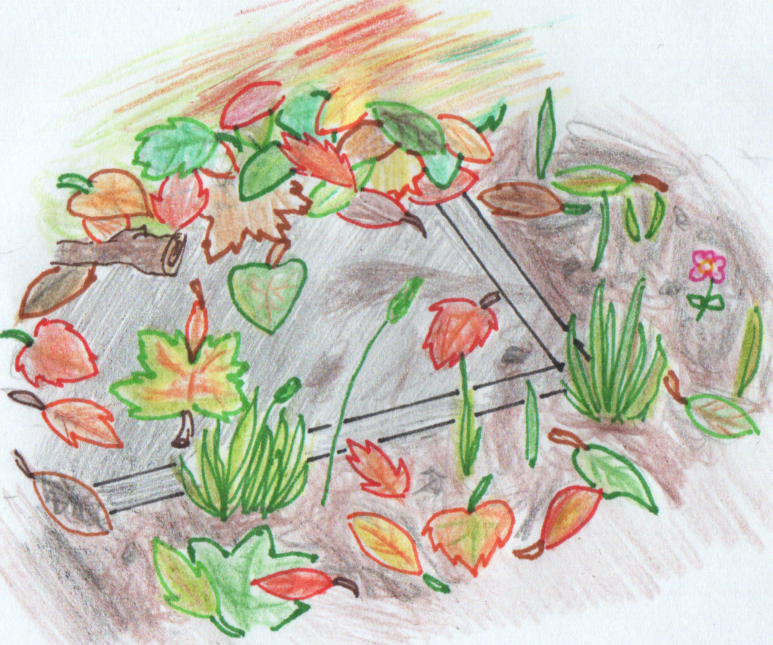
\includegraphics[scale=0.7]{Bilder/luke1.png}
  \caption{Die geheimnisvolle Luke}
\end{figure}


\chapter{Beweis} %bis 2.6
\begin{chapquote}{Sören Kierkegaard}
\glqq Oder ist etwa Schwermut nicht das Gebrechen der Zeit, ist sie es nicht, die selbst in deren leichtsinnigem Gelächter widerhallt?\grqq
\end{chapquote}

%2.3
\textit{Der 10. Mai 2020} \\
     
\parasep

%2.4
     
\parasep

%2.5
Der Kassettenspieler fing zu surren an und bald darauf zeigte der angeschlossene Fernseher statisches Grau. Die Jugendlichen betrachteten einander schweigend, aber mit eindringlichen und besorgten Blicken. Das Bild richtete sich und zeigte bald daraufhin zum Erstaunen der Allgemeinheit eine Tagesschausendung. Der bekannte Gong schlug, um anzuzeigen, dass es 20 Uhr war. Patrick schnaubte.
„Was machen wir hier eigentlich?“ \\
„Sshht“, wies ihn Christian zurecht. Er starrte gebannt auf den Bildschirm. Die bekannte Intromusik spielte ab und die Moderatorin wurde vorgestellt, die den Zuschauern die wohl hunderte Male eingeübten Begrüßung aufsagte. \\
„Deutschland überschreitet die Marke von 300.000 Coronainfektionen – Bund und Länder debattieren über strengere Maßnahmen“ lautete die erste Überschrift. Es wurden Ausschnitte aus Interviews mit Vertretern der Parteien des deutschen Bundestages abgespielt. Veran wurde ganz blass. \\
„Waren das gestern nicht noch um die 170.000?“, fragte er mit zitternder Stimme. Keiner seiner Freunde wusste eine Antwort. Weitere Coronamaßnahmen wurden vorgestellt, die die Jugendlichen nur noch mehr verblüfften. Als die drastische Coronasituation in Serbien thematisiert wurde, konnte sich Sofia ein geschocktes Aufatmen nicht verkneifen. Anschließend ging es um die allgemeine Lage der Wirtschaft sowie um ein Attentat auf einen FDP-Politiker. \\
„Der thüringische FDP-Spitzenkandidat Kemmerich befindet sich außer Lebensgefahr. Der Verdächtige, ein siebzehnjähriger chinesischer Staatsbürger namens Y. Yang, ließ sich widerstandslos festnehmen.“ \\
„Was sind das für seltsame Nachrichten?“, empörte sich Sofia. Doch was folgte, sollte ihnen allen die Haare zu Berge stehen lassen. Die Sprecherin setzte zu ihrem nächsten Satz an. \\
„Die deutsche Mannschaft für die Internationale Mathematikolympiade musste heute bei der Veröffentlichung der Ergebnisse des dezentral ausgeführten Wettbewerbes eine beispiellose Blamage hinnehmen. Mit zwei von insgesamt 252 erreichbaren Punkten erzielte sie ein historisch schlechtes Ergebnis und wurde so zur Zielscheibe internationaler Kritik.“
Die Sendung schnitt zu einem asiatisch aussehenden jungen Mann, der etwas in ein Mikrofon sagte. Unten am Bildschirm wies ihn ein eingeblendetes Schild als „Evan Chen – Koordinator IMO“ aus. \\
„This result is truly a disgrace“, sagte er angespannt in die Kamera, während er rot anlief. Eine blaue, pulsierende Ader an seiner Schläfe stach hervor. „The quality of the returned papers was unlike anything I had seen before.“ Er rückte seine Krawatte zurecht und blickte vorwurfsvoll in die Kamera. Er schien sich nur schwer zurückhalten zu können. „I will \textit{not} let the image of the IMO be treated like this, Dr. Prestin! You will PAAAY!“ Er schlug das Mikrofon des Reporters beiseite und schien auf jemanden hinter der Kamera losgehen zu wollen, als er mit Mühe von zwei Sicherheitskräften festgehalten wurde. Nun wurde zurück ins Studio geschaltet. Die Moderatorin schaute kurz auf ihre Notizen. \\
„Das Komitee entschied, Deutschland in Zukunft von der Internationalen Mathematikolympiade auszuschließen, da eine solche abysmale Leistung nicht dem Charakter der IMO entspräche. Dem deutschen Teamleiter Dr. Jürgen Prestin wurden weiterhin seine Medaillen aberkannt. Unter riesigem öffentlichem und auch innerakademischem Druck gab dieser seine Professur an der Universität zu Lübeck auf und zog sich aus dem öffentlichen Leben zurück.“ \\
„Das können die doch nicht ernst meinen“, entfuhr es Patrick unwillkürlich. Die restlichen Anwesenden waren wie versteinert. Maria wollte etwas sagen, als die Sprecherin wieder das Wort ergriff. \\
„Und nun die Wettervorhersage für morgen, Sonntag, den 27. September 2020.“

     
     \parasep
     %2.6
     
Im Raum war es sehr ruhig. Keiner schien sich wirklich von dem Schock erholt zu haben. Keiner wusste, wie er mit der Situation umgehen sollte. 
In den Köpfen der Jugendlichen vermischten sich alle möglichen Gedanken.
Maria war völlig verwirrt. War das gerade wirklich echt? Wie konnten sie Daten aus der Zukunft sehen?
Veran kam das vor wie in einem Horrorfilm. Er hoffte, dass das ganze nur ein schlechter Traum war. Doch das war es leider nicht\ldots
Sofia war überfordert; das war einfach zu viel für sie. Am meisten beschäftigte sie jedoch, dass ihr Lieblingsland Serbien in der Sendung vorgekommen ist.
Georgi hatte ein schlechtes Gefühl. Vielleicht durften sie gar nicht in dem Keller sein? Vielleicht war das ein höchst geheimer Ort, der dem Forschungsinstitut gehört, und der sie nichts anging? Und doch war er sich ziemlich sicher, dass das alles mit dem Verschwinden der zwei AIMO-Teilnehmer zu tun haben könnte\ldots

Alle schwiegen. Niemand traute sich, was zu sagen. Jeder stand in seiner eigenen Ecke und bewegte sich nicht.
Auf einmal hörte man die Stimme von Patrick. \\
„Jungs, wisst ihr was? Ich hab‘ keinen Bock mehr auf die Scheiße! 
Ich geh‘ wieder zurück.“
Alle waren verwundert und auch ein wenig enttäuscht von Patricks desinteressierter Einstellung, aber keiner versuchte, irgendwas zu machen, und er wurde einfach gehen gelassen.

So blieben sie nur noch zu viert im dunklen Keller und schwiegen weiterhin kurz, bis Veran dann sagte:  \\
„Ich glaub Patrick hatte Angst. Deswegen ist er abgehauen.“ \\
„Richtiger Alman-Move\ldots“, sagte Sofia darauf. \\
„Ich finde, wir sollten nicht aufgeben“, äußerte sich Georgi wenige Sekunden später. „Ich\ldots{} ich glaube, Christian könnte gerade hier sein.“

Allmählich kam jeder der vier wieder zu sich und sie erkundeten weiter zusammen den Keller.
In einer Ecke befand sich eine Tür, die jeder beim Reingehen sofort gemerkt, sich ihr anzunähern sich aber keiner getraut hatte.  \\
„Wir müssen da durch. Es bleibt uns nichts Anderes übrig“, befiel Georgi.
Und so gingen die vier in Richtung dieser Tür.
Sofia stand als Erste vorne und drückte die Klinke herunter. Die Tür öffnete sich. Hinter ihr befand sich ein weiterer Raum. Sie drückte auf den Lichtschalter. Sie schaute unter sich.
Auf einmal hörte man einen lauten Schrei.
Die anderen drei kamen sofort zu ihr. Sie schauten herunter und glaubten nicht was sie sahen. Dann schauten sie sich gegenseitig an. \\
„Ist \ldots{} ist das \ldots{} Marc?“, fragte Maria ängstlich.
Tatsächlich lag auf dem Boden, unter sehr vielen Mathe-Arbeitsblättern,
der Körper von Marc. Seine Haut war völlig blass. Er war ohnmächtig geworden. \\
„Wir müssen schnell handeln“, sagte Veran unruhig. „Maria, ruf einen Notarzt an!“
Alle zusammen trugen den Körper die Treppe hoch. Maria musste etwas weiter weg vom Keller gehen, um nach Netz zu suchen. Die anderen drei blieben bei der Treppe. Veran blieb -- aus Angst herunterzufallen -- am unteren Teil der Treppe.
Und dann erkennte er im hinteren Teil des Kellers eine ihm bekannt vorkommende Person. Sie kam immer näher. \\
„Georgi, Sofia, kommt schnell!“, rief Veran. Die drei gingen schnell in den anderen Raum. Sie wussten sofort alle, um wen es sich handelte. \\
Es war Christian. \\
Er wirkte jedoch recht zurückhaltend, als die anderen auf ihn zugingen. \\
„Ihr dürft hier nicht sein“, sagte er. \\
„Wir sind hier, um dich rauszuholen“, erklärte Georgi. \\
„Geht raus! Er kommt gleich.“ \\
„Wer kommt gleich??“ fragte Veran.
Zögernd antwortete Christian: \\
„Herr Prestin.“

\chapter{Rückbezug} %bis 3.1
\begin{chapquote}{Veran Stojanović}
\glqq Was wir wissen, ein Epsilon. Was wir nicht wissen, ein 1/Epsilon.\grqq
\end{chapquote}

\chapter{Abschließende Überlegungen} %bis 4.2
\begin{chapquote}{Veran Stojanović}
\glqq Wie kommt man zum Höhepunkt?\grqq
\end{chapquote}
„\ldots{} und deshalb werde ich hier seit 2 Wochen gezwungen, nur Mathe zu machen.“ \\
Sofia, Georgi und Veran hatten Christian überredet, ihnen alles zu erzählen. Sie konnten es nicht fassen, was in den letzten Tagen in diesem Keller abging. \\
„Also\ldots{} dieser Herr Prestin, der das alles gemacht hat, kommt\ldots{} ähm\ldots{} aus der Zukunft?“, fragte Sofia verwirrt. \\
„Ja\ldots“, antwortete Christian. „Ich konnte das am Anfang auch nicht fassen.“ \\
„Und er wollte das IMO-Ergebnis verbessern, indem er in die Vergangenheit reist, einen potenziellen Teilnehmer in einen Keller einsperrt, und ihn auf brutale Weise dazu zwingt, Mathe zu machen?? Der Typ ist ein Psychopath!“ sagte Veran wütend. \\
„Ach komm! Man muss schon ein bisschen Mitleid mit ihm haben. Er hat ja schließlich alles verloren\ldots{} Und außerdem find‘ ich’s mittlerweile ganz okay hier. Ich mein‘\ldots{} ich mach‘ ja den ganzen Tag Mathe, besser geht’s doch nicht!
Ach ja, und der Sonntagsbraten von Herr Prestin ist der Beste, den ich je gegessen hab‘!“ \\
„Christian, was redest du eigentlich gerade???“, schrie ihn Georgi an. „Schau dich mal an! Du bist völlig blass geworden! Das, was Herr Prestin mit dir und Marc gemacht hat -- und wahrscheinlich bald mit anderen AIMO-Teilnehmern machen wird -- ist äußerst strafbar! Wir müssen die Polizei anrufen.“ \\
In dem Moment erschien aus einer Tür im anderen Raum Herr Prestin. \\
„Oh! Herr Kocharyan! Frau Zotova! Herr Stojanović! Das ist ja niedlich!“ \\
„Wir wissen alles!“, konfrontierte ihn Georgi. „Wie konnten Sie nur zwei Jugendliche entführen und sie in einen Keller einsperren? Und das alles um Ihren scheiß Ruf nicht zu verlieren! Wissen Sie was? Mich interessiert gar nicht wie intelligent Sie sind und was Sie alles bisher erfunden und entdeckt haben. Aber eine so mächtige wissenschaftliche Erkenntnis für solche dumme Sachen zu missbrauchen\ldots{} dafür sollten Sie sich wirklich schämen!!!“ \\
„Jetzt haben Sie doch ein wenig Mitleid mit mir. Ich wollte das nur für unser IMO-Team machen\ldots“, rechtfertigte sich Herr Prestin. Nach kurzem Überlegen sagte er: „Okay. Entschuldigung. Vielleicht habe ich wirklich etwas übertrieben. Ich verspreche, das nie wieder zu machen. Können wir jetzt damit leben?“  \\
Sofia, Georgi und Veran schauten sich kurz an und dann sagte Georgi: 
„Nein. Wir vergeben Ihnen nicht. Sie müssen zur Polizei.“ \\
Herr Prestin ließ sich schließlich zwingen, die Treppe hochzugehen. Man erkannte in seinem Gesicht eine tiefe Traurigkeit -- er hat nicht das geschafft, was er wollte. Er sagte dann noch einen letzten Satz zu Christian. \\
„Herr Noaghiu, geben Sie bitte alles bei der IMO. Ich weiß, dass Sie das können.“ \\
Und so gingen sie zu fünft aus dem Keller heraus. Die Polizei hatten sie bereits kontaktiert. 
Und dann hörte man ein lautes Geräusch, gefolgt von einem lauten Schrei. Veran war beim Hochgehen gestolpert und die Treppe heruntergefallen. Christian, Sofia und Georgi eilten schnell zu ihm hinunter. \\
„Alles okay?“ \\
Zum Glück hatte er nur eine kleine Wunde. Er hatte sich aber so sehr erschreckt, dass er Angst hatte, wieder hochzugehen. Mit vereinten Kräften schafften es die anderen, ihn dazu zu bringen, die Treppe wieder zu besteigen. \\
„Es ist nur eine dumme Treppe. Das wird nie wieder passieren“, ermutigten sie ihn.
Und gerade als sie bereit waren wieder hochzugehen, erblickten sie Herrn Prestin, wie er ein Morley-Dreieck in der Luft erscheinen ließ. Und schon war er hindurch verschwunden.  \\
„Jebiga“, fluchte Sofia.

\parasep
     %4.2
     
„Das kann er doch nicht ernst meinen!“ Georgi war außer sich vor Wut. „Und was machen wir jetzt?“ \\
„Also ich will einfach nur hier raus!“, sagte Christian.
Das ließen sich die anderen nicht zweimal sagen. Und so stiegen sie gemeinsam die Treppe hinauf -- Veran hatte dabei immer noch ein mulmiges Gefühl -- und verließen das dunkle Gewölbe über die Luke. \\
„Frische Luft!“, rief Veran begeistert.
Es war inzwischen Nacht geworden. Über dem Wald ruhte der Vollmond, der die Umrisse der Bäume sichtbar machte. Ganz leise war im Hintergrund der Gesang einer Nachtigall zu vernehmen.
Die Stimmung war ungewöhnlich. Nicht gruselig – so wie das erste Mal, als die Jugendlichen hier gewesen waren. Und doch lag etwas in der Luft. Die vier hatten unglaubliche Dinge gesehen. Was würden nur die anderen Teilnehmer dazu sagen? \\
Als sie in Richtung des Instituts zurückgingen, kam auf einmal eine Gestalt auf sie zu. \\
„Patrick!“, rief Christian, „Wo kommst du denn her?“ \\
„Jungs“, schnaufte Patrick darauf. „Ich weiß Bescheid. Wir müssen sofort zu Prestin.“
Sofia war verwundert. \\ „Hä Patrick, Prestin ist vorhin vor unseren Augen verschwunden! Lass mal lieber zu den anderen ins Institut gehen!“
Doch Patrick ließ nicht locker.  \\
„Es geht um Zeit. Zeit ist alles! Passt auf: Prestin ist aus der Zukunft zurückgekommen. Dieser Prestin ist aus der Zukunft. Es gibt aber noch den ‚richtigen‘ Prestin von jetzt, der sich in der Zukunft dazu entscheiden wird, zurückzureisen und das alles anzurichten. Und das ist unsere einzige Chance: Wir müssen den Prestin von jetzt genau daran hindern. Dann wird er nicht zurückreisen, und der Zukunftsprestin von jetzt wird nie existiert haben. Versteht ihr?“
Sofia war verwirrt. \\
„Fishy. Ich versteh‘ gar nichts mehr – wir verändern die Zukunft, damit in der Vergangenheit, die ja dann die Gegenwart ist – nein, wir verändern die Gegenwart, damit in – ach, das ist viel zu kompliziert!“
Doch Veran schien zu begreifen. \\
„Das ist echt big brain“, meinte er zu Patrick. „Aber was sagen wir denn jetzt zu Prestin? ‚Sie werden sich in der Zukunft dazu entschließen, durch die Zeit zu reisen, um AIMO-Teilnehmer einzusperren‘? Das glaubt er uns nie im Leben!“
Aber auch dafür wusste Patrick einen Rat. \\
„Wir haben Beweise: seine Akten und die Kassette. Und das er durch die Zeit reisen kann, weiß er schon seit über 30 Jahren.“
Die anderen stimmten ihm zu. \\
„Okay, auf zu Prestin“, forderte Christian die anderen auf. \\
„Moment mal, wo ist Maria?“, unterbrach ihn Sofia.
„Wir haben keine Zeit. Prestin ist in seinem Zimmer, wir müssen uns beeilen“, antwortete Patrick knapp. \\
„Sag mal, Patrick“, holte Georgi aus. „Woher weißt du das alles?“ \\
„Das spielt jetzt keine Rolle. Wir müssen los.“ \\
Und so rannten die fünf Jugendlichen los, bogen kurz vor dem Institut ab und näherten sich stattdessen dem Hotel. Sie öffneten die Tür, stiegen mit schnellen Schritten die Treppe hinauf und betraten den Gang, in dem die Mentoren wohnten. Patrick suchte nach der Zimmernummer von Herrn Prestin. \\
„39, 40, 41, 42. Hier ist es!“
Er hielt kurz inne, nahm allen Mut zusammen und öffnete die Tür. \\
„Herr Prestin!“, rief Sofia – aber er lag bereits in seinem Bett und schlief. \\
„Mist“, flüsterte Georgi darauf enttäuscht, „Wollen wir ihn wecken?“ \\
„Ne, lass mal nicht“, meinte Veran.
Doch dann spürten die Jugendlichen plötzlich in ihren Nacken einen tiefen Blick, der sie durchbohrte. Einer nach dem anderen drehten sie sich um und erblickten Jan-Christoph Schlage-Puchta, der wie aus dem Nichts in der Tür erschienen war. Er wirkte nicht erfreut, sie zu sehen – geradezu bedrohlich. \\
„Na, wen haben wir denn da?“, sagte er mit einem breiten Grinsen im Gesicht. Kurz darauf sahen die Jugendlichen nur noch verschwommen, und nach wenigen Sekunden wurde alles schwarz.

     
     
\chapter{Im Kerker} %bis 4.3
\begin{chapquote}{Paul Pelisson}
\glqq Grandeur, savoir, renommée, \\
Amitié, plaisir et bien, \\
Tout n’est que vent, que fumée, \\
Pour mieux dire, tout n’est rien.\grqq
\end{chapquote}

Allmählich wachten die Jugendlichen auf und kamen zu sich. Ihnen dröhnten die Köpfe. Sie schauten sich um und bemerkten, dass sie an einem anderen Ort waren. Schnell bemerkten sie, um welchen Ort es sich handelte. Sie waren in Prestins Keller, allerdings in einem kleineren Raum, der ihnen nicht bekannt war. \\
„Oh Gott, was machen wir hier?“, ächzte Georgi. 
Sofia sprang auf und lief zu der vergitterten Tür. Sie versuchte, gegen das Gitter zu drücken, am Ende schlug sie sogar verzweifelt gegen die Tür. \\
„Lasst uns heraus!“, schrie sie verbittert. Nach einigen Minuten setzte sie sich wieder zu den anderen. \\
Patrick zeigte auf einen seltsam aussehenden Kasten, der in einer Ecke stand. \\
„Was ist das denn?“ \\
„Damit findet Herr Prestin heraus, ob du bereit für die IMO bist“, antwortete Christian. „Er nennt es den Prestindikator.“ \\
„Aaar.“ \\
Einige Sekunden vergingen in Stille, bis Veran etwas sagte. \\
„Ich glaube, das, was gerade abgeht, ist viel größer, als wir denken. Wie eine riesige Verschwörung. Und wir können den Lauf der Dinge nicht ändern. Das hier ist auch Teil unseres Schicksals.“ \\
Christian saß nur alleine in einer Ecke und summte vor sich hin. Als die anderen das hörten, stimmten sie, vielleicht um der betrübten und ernsten Stimmung entgegenzuwirken, ein Lied an. \\


\begin{singlespace}
\noindent 
\glqq In the time, when I was born \\
Lived a man, who swinged through time \\

\noindent 
And he told us of first life \\
In the fall of twenty-nil \\

\noindent
So we wandered, through the night, \\
till we found, the hidden hatch \\

\noindent
And we lived, beneath the ground, \\
in the cellar, of Prestin \\

\noindent 
We all live in the cellar of Prestin \\
Cellar of Prestin \\
Cellar of Prestin \\
We all live in the cellar of Prestin \\
Cellar of Prestin \\
Cellar of Prestin \\

\noindent 
And our friends are all aboard \\
Many more of them, locked next door \\

\noindent 
And the Zoom meeting begins \\
da da di dum di dum di dum \\

\noindent 
We all live in the cellar of Prestin \\
Cellar of Prestin \\
Cellar of Prestin \\
We all live in the cellar of Prestin \\
Cellar of Prestin \\
Cellar of Prestin \\

\noindent 
And we lived a life of math \\
Many triangles is all we have \\ 

\noindent 
Lines of tears and points of blood \\
In the cellar, life is hard \\ 

\noindent 
We all live in the cellar of Prestin \ldots\grqq
\end{singlespace}

„Schade, dass Maria nicht da ist“, seufzte Sofia. „Die Beatles sind doch ihre Lieblingsband.“ \\
„Leute, was ist das?“, fragte Georgi auf einmal. \\
„Die Beatles?“, antwortete Sofia verwirrt. \\
„Nein, schau doch hinter dir!“ \\
Eine majestätisch violett leuchtende Form schwebte in der Luft. Ein Dreieck. Die Jugendlichen starrten es verwundert an. \\
„Ein Morley-Dreieck!“, rief Patrick. Doch dann wurden die Höhen auf den drei Seiten langsam eingezeichnet. \\
„Das ist kein Morley-Dreieck“, sagte Veran. \\
Es ergab sich eine Figur, deren Existenz sie nie für möglich gehalten hätten. \\
„Was zum \ldots?! Warum schneiden die Höhen sich nicht in einem Punkt?“, schrie Sofia aufgebracht. Das kleine Dreieck in der Mitte, das von den drei Höhen gebildet wurde, leuchtete auf. Dessen grelles Licht wurde fast unerträglich. Doch dann hörte man jemanden sprechen. \\
„Kommt her!“, sagte er direkt aus dem Höhendreieck. Die fünf schauten sich an, diesmal völlig aus der Fassung. \\
„Ich kenne diese Stimme“, sagte Sofia leise, und auch alle anderen verstanden, um wen es sich handelte. „Das ist doch nicht\ldots“ \\
Eine Hand erschien durch das Höhendreieck und Max Keßler rief: „Jetzt beeilt euch, wir haben nicht mehr viel Zeit!“ \\
Die Jugendlichen wussten, was zu tun war. Nachdem sie sich zugenickt hatten, griffen sie gleichzeitig nach seiner Hand. Und sobald ihre Hände sich berührt hatten, waren sie mitsamt des Dreiecks verschwunden.
\newpage
\thispagestyle{empty}
\begin{center}
\textit{Fortsetzung folgt\ldots}
\end{center}

\chapter{Anhang}
\begin{chapquote}{Veran Stojanović}
\glqq Wenn Max Keßler uns rettet, ist es ein deus ex maxina.\grqq
\end{chapquote}
\section*{Honourable Mentions für den Titel}
\begin{itemize}
\item Prestinhaftiert
\item Under Presture
\item Pressed In
\item Trabbel in Oberwolfach
\item In Jürgens Keller
\item Der unendliche Abstieg
\item Prestinfiziert
\item Prestissimo
\item Presto ma non troppo
\item Abschwung
\item Prestinternationale Mathematik-Olympiade
\end{itemize}
\section*{Fachbegriffeglossar}
% i.t.s, Yarrack, Jebiga, ölen, Höhendreieck, Morleydreieck
\paragraph{Jebiga.} Serbischer vulgärer Ausdruck, der mit „verdammt“, „was solls“ oder „Pech gehabt“ übersetzt werden kann. Mit dem Ausdruck „Jebiga“ wird Resignation und das Akzeptieren von unveränderlichen Fakten oder Lebensumständen ausgedrückt.
\paragraph{Ölen.} Ist kein Brokkoli
\paragraph{Yarrack-Formel.} siehe \url{https://www.youtube.com/watch?v=LJVH4_HBTrw}
\paragraph{Höhendreieck.}  Das Dreieck, das durch die drei Höhen eines größeren Dreiecks entsteht, wenn sie sich nicht in einem Punkt schneiden.
\paragraph{Morleydreieck.} Das gleichseitige Dreieck, das durch die drei Winkeldreiteilenden eines anderen Dreiecks aufgeschwungen wird. Durch eine Fehlinterpretation der Aussage „es verschwinden Dinge während des Vortrags  über das Morleydreieck“ kam es zum Mythos über das Zeitreisen.
\paragraph{Sonntagsbraten.} Äußerung J. Prestins während eines Zoomseminars, die Teilnehmer würden sich auf den Sonntagsbraten freuen.
\paragraph{i.t.s.} nordrhein-westfälische Wendung für „immediate to see“
\paragraph{Vizepräsident Vučić.} prominenter serbischer Politiker
\paragraph{Chaya.} weibliche Form von Jiggo
\paragraph{Nummernachbar.} Eine Person, dessen Telefonnummer sich in der letzten Ziffer von der eigenen unterscheidet. Geschehnisse in der Fanfiction basieren auf realen Ereignissen, wo Patrick von seinem Nummernachbar namens Michael mit wirren Nachrichten angeschrieben wurde.
\paragraph{(Dickes) mal sehen.} Synonym zu „auf keinen Fall“.
\newpage
\section*{Danksagung} 
Wir bedanken uns bei allen Teilnehmern und Mentoren der AIMO 2020 für die unglaublich schöne Zeit, die wir auf den Seminaren verbringen durften. Nachdem wir uns dort kennengelernt hatten, haben wir nicht nur auf den Seminaren, sondern auch in unserer Freizeit wir viel Zeit miteinander verbracht und konnten eine wirklich enge Freundschaft schließen -- danke, dass uns hierfür der Anlass geboten wurde. \\
Wir wünschen allen Teilnehmern alles Gute für die Zukunft und fürs Studium, und weiterhin der IMO-Mannschaft (insbesondere Christian Noaghiu, der sehr intensiv dafür traniert hat) viel Erfolg!

\end{document}
